\documentclass[12pt,aspectratio=169]{beamer}
\usetheme{default}
\usecolortheme{dolphin}
\usefonttheme{structurebold}
\setbeamertemplate{footline}[frame number]

\title{Network 04}
\author{@aoirint}
% \institute{}
\date{2020/05/28}

\begin{document}

% 01
\frame{\maketitle}

% 02
\begin{frame}{テキスト}

  \begin{minipage}{0.58\textwidth}
    \begin{itemize}
      \item ネットワークがよくわかる教科書
      \begin{itemize}
        \item 著・福永勇二
        \item 刊・SB Creative
      \end{itemize}
      \item 今回の内容
        \begin{itemize}
          \item Chapter 2、Section 9から12まで
        \end{itemize}

    \end{itemize}

  \end{minipage}
  \hfill
  \begin{minipage}{0.38\textwidth}
    \vspace{-1\baselineskip}
    \begin{figure}[h]
      \centering
      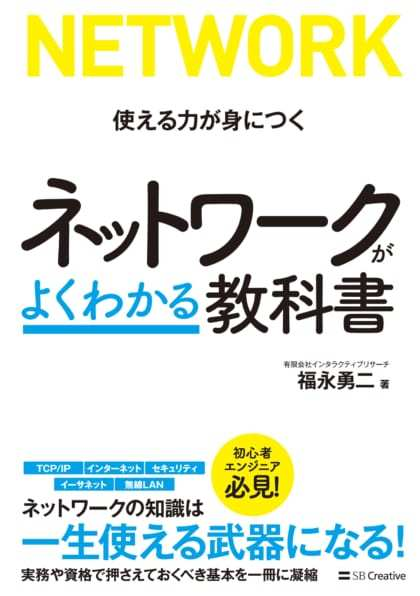
\includegraphics[width=4cm,bb=0 0 420 596]{../02/figures/networkbook.jpg}
      \label{fig:networkbook}
      \caption{テキスト}
    \end{figure}
  \end{minipage}

  \begin{itemize}
    \item 書影
    \begin{itemize}
      \item { \small \url{https://www.sbcr.jp/product/4797393804/} }
    \end{itemize}
  \end{itemize}

\end{frame}


\begin{frame}{今回の内容}

  \begin{itemize}
    \item 基本的なパケットのフォーマット
      \begin{itemize}
        \item IPパケットのフォーマット(復習)
        \item TCPパケットのフォーマット(復習)・チェックサム計算
        \item UDPパケットのフォーマット
      \end{itemize}
    \item ネットワークにおける通信
      \begin{itemize}
        \item ARPの機能とパケットのフォーマット
        \item パケットの送受信処理の概観
        \item ルーティングテーブルの役割
        % \item IPパケットの分割と再構築
      \end{itemize}

  \end{itemize}

\end{frame}


\begin{frame}{IPパケットのフォーマット(復習)}

  \centering
  \begin{figure}
    \centering
    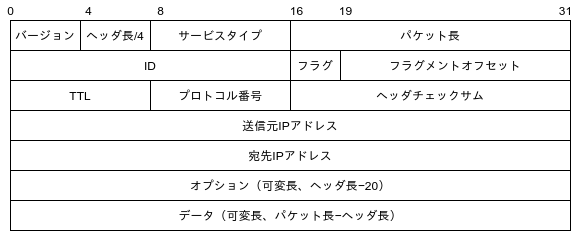
\includegraphics[width=12cm,bb=0 0 581 232]{./figures/ip_packet.png}
    \label{fig:ip_packet}
    \caption{IPパケットのフォーマット(IPv4)}
  \end{figure}

\end{frame}


\begin{frame}{TCPパケットのフォーマット(復習)}

  \centering
  \begin{figure}
    \centering
    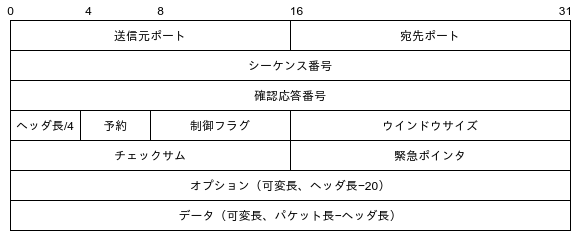
\includegraphics[width=12cm,bb=0 0 581 231]{./figures/tcp_packet.png}
    \label{fig:tcp_packet}
    \caption{TCPパケットのフォーマット}
  \end{figure}

\end{frame}


\begin{frame}{TCP/IPパケット}

  \centering
  \begin{figure}
    \centering
    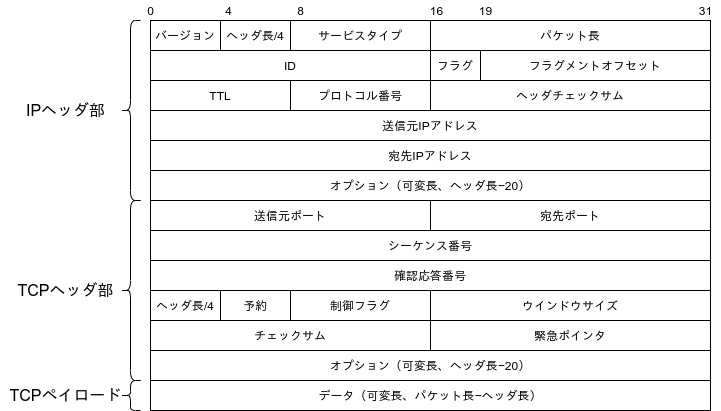
\includegraphics[width=12cm,bb=0 0 721 411]{./figures/tcpip_packet.png}
    \label{fig:tcpip_packet}
    \caption{TCP/IPパケットのフォーマット(IPv4)}
  \end{figure}

\end{frame}


\begin{frame}{TCPチェックサムの計算 1/2}

  \begin{itemize}
    \item TCPのチェックサム計算にはIPアドレスを含める
    \item TCP擬似ヘッダ:TCPに対する擬似的な上位層のヘッダ(IPアドレス情報)
      \begin{itemize}
        \item IPヘッダに相当するもの
      \end{itemize}
  \end{itemize}

  \centering
  \begin{figure}
    \centering
    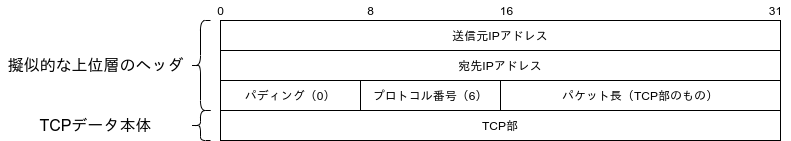
\includegraphics[width=12cm,bb=0 0 791 141]{./figures/tcp_pseudo_header.png}
    \label{fig:tcp_pseudo_header}
    \caption{TCP擬似ヘッダ(IPv4)}
  \end{figure}

\end{frame}


\begin{frame}{TCPチェックサムの計算 2/2}

  \begin{itemize}
    \item TCP擬似ヘッダ・TCPヘッダ・TCPデータ部について、16ビットごとの1の補数和をとった値の1の補数
    \item TCPヘッダのチェックサム部は0として計算
    \item 1の補数和
      \begin{itemize}
        \item 最上位ビットの桁上がりを最下位ビットに足す
        \item 0b0110 + 0b0011 = 0b1001(最上位ビットの桁上がりなし)
        \item 0b1000 + 0b1000 = 0b0001(最上位ビットの桁上がり)
        \item 0xF000 + 0x1000 = 0x0001(16ビット=2バイト)
      \end{itemize}
    \item ある値の1の補数をとる
    \begin{itemize}
      \item 補数:ある値と和をとったとき0になる数
      \item 1の補数では論理否定をとると補数
      \item チェックサムに対してもう一度パケット全体の1の補数和を計算して足し合わせると0になる
    \end{itemize}

    \item ref: \url {https://www.wdic.org/w/SCI/1\%E3\%81\%AE\%E8\%A3\%9C\%E6\%95\%B0}
  \end{itemize}

\end{frame}


\begin{frame}{UDPパケットのフォーマット}

  % \begin{itemize}
  %     \item
  % \end{itemize}

  \centering
  \begin{figure}
    \centering
    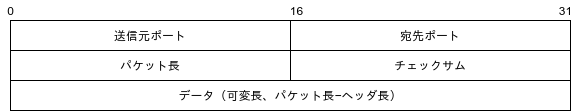
\includegraphics[width=12cm,bb=0 0 581 111]{./figures/udp_packet.png}
    \label{fig:udp_packet}
    \caption{UDPパケットのフォーマット}
  \end{figure}
\end{frame}


\begin{frame}{UDPチェックサムの計算}

  \begin{itemize}
    \item 計算方法はTCPと同じ(16ビットごとの 1の補数和の 1の補数)
    \item プロトコル番号:17(UDP)
  \end{itemize}

  \centering
  \begin{figure}
    \centering
    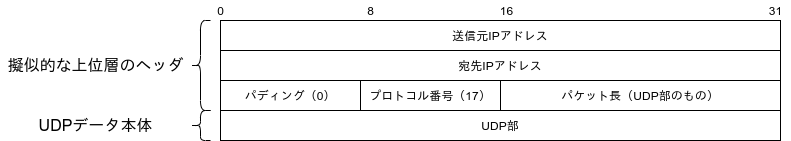
\includegraphics[width=12cm,bb=0 0 791 141]{./figures/udp_pseudo_header.png}
    \label{fig:udp_pseudo_header}
    \caption{UDP擬似ヘッダ(IPv4)}
  \end{figure}
\end{frame}


\begin{frame}{ARP / Address Resolution Protocol 1/3}

  \begin{itemize}
    \item 異なるネットワークとの通信(インターネット層)
      \begin{itemize}
        \item IP:論理アドレス(ルータを介して通信)
        \item IPを使って相手のネットワークにまでパケットを届けることはできる
      \end{itemize}
    \item 同一ネットワーク内の通信(ネットワークインタフェース層)
      \begin{itemize}
        \item Ethernet:物理アドレス(L2スイッチを介して通信)
        \item ルータは外部から届いたパケットをネットワーク内のどのホストに送ればいいか判断する必要がある
        \item 送信元ホストは同一ネットワークにいる、ある論理アドレスのホストの物理アドレスを知る必要がある(L2スイッチを介した通信をイメージ)
        % 空欄にしておいてルータが処理すればいいじゃないか、と思うかもしれないが
      \end{itemize}
    \item ルータや送信元ホストは、宛先ホストの論理アドレスと物理アドレスの対応表を持つ必要がある
      \begin{itemize}
        % 静的に管理していたら、NICの破損などに対応できるように
        % 論理アドレスを設定している意味がないから、
        % 動的に取得するのがよいということになる
        % そのための通信プロトコル
        \item ARP:Address Resolution Protocol
      \end{itemize}

  \end{itemize}

\end{frame}


\begin{frame}{ARP / Address Resolution Protocol 2/3}

  \begin{itemize}
    \item ブロードキャスト
      \begin{itemize}
        \item ネットワーク内の全ホストにパケットを送る
        \item ブロードキャストを表す物理アドレス:FF:FF:FF:FF:FF:FF
      \end{itemize}
    \item ARPリクエスト
      \begin{itemize}
        \item 対応する物理アドレスを知りたい論理アドレスをパケットに含めてブロードキャスト
      \end{itemize}

    \item ARPリプライ
      \begin{itemize}
        \item ARPリクエストの受信者は自分の使っている論理アドレスと照合
        \item 一致していれば送信者に応答して物理アドレスを明らかにする
      \end{itemize}

    \item ARPキャッシュ
      \begin{itemize}
        \item 端末やルータで物理アドレスと論理アドレスの対応を一時的に保存する
        \item ARPリクエスト数を減らす
      \end{itemize}

  \end{itemize}

\end{frame}


\begin{frame}{ARP / Address Resolution Protocol 3/3}

  \begin{itemize}
    \item HLEN:ハードウェアアドレス長(物理アドレス長)
    \item PLEN:プロトコルアドレス長(論理アドレス長)
    \item arp -a
  \end{itemize}

  % 実際には応用が効くように一般化されてるらしいけどイーサネットの場合はこの構造
  % ARPリクエスト時の宛先MACアドレスは適当な値でいい(実際には上位層であるイーサネットヘッダのMACアドレスにブロードキャストアドレスを指定して、それが使われるから)
  % 実はイーサネットのデータ部の最小サイズは46バイトで、ARPは28バイトしかない、残りはパディングとしてダミーデータを入れて埋める
  \centering
  \begin{figure}
    \centering
    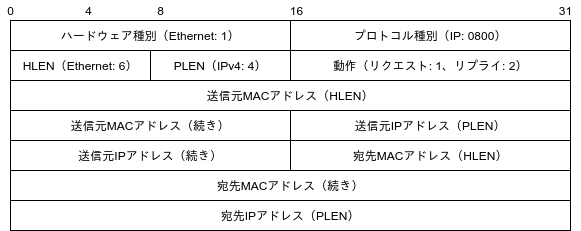
\includegraphics[width=12cm,bb=0 0 581 231]{./figures/arp_packet.png}
    \label{fig:arp_packet}
    \caption{ARPパケット(イーサネット)}
  \end{figure}

\end{frame}

% TCPパケットを例にパケットの送受信処理の概観を見ていく
\begin{frame}{パケットの送受信処理:同一ネットワーク内 1/2}

  \begin{itemize}
    \item 同じイーサネットにつながる端末同士の通信
    \vspace{0.5cm}
    \item アプリケーションメッセージ(アプリケーション層のデータ)
    \item TCPによるパケット分割
      \begin{itemize}
        \item MTU / Maximum Transmission Unit
          \begin{itemize}
            \item ネットワークハードウェアから決まる適切なパケットサイズ(パケット全体)
          \end{itemize}
        \item MSS / Maximum Segment Size
          \begin{itemize}
            \item TCPパケットのデータ部の適切なサイズ
            \item MSS = MTU - 20(TCPヘッダ) - 20(IPヘッダ)
            \item 通信相手と接続処理時に交換して小さい方を使う
          \end{itemize}
      \end{itemize}
    % TCPですでに適切なサイズに分割しているのでTCPの場合は行われないと思うが、一応
    \item (IPによるパケット分割(フラグメンテーション))
  \end{itemize}

\end{frame}

\begin{frame}{パケットの送受信処理:同一ネットワーク内 2/2}

  \begin{itemize}
    \item IPヘッダの付加
    \item ARPにより論理アドレスから宛先MACアドレスを取得
    \item イーサヘッダの付加、イーサフレームとして送出
    \vspace{0.5cm}
    \item 受信、宛先MACアドレスを確認、自分と一致していなければ破棄(無視)
    \item イーサフレームを検査、イーサヘッダを除去
    \item IPパケットを検査、IPヘッダを除去(、IPによる分割の再構築)
    \item TCPパケットを検査、アプリケーションメッセージの再構築
    \item アプリケーションがデータを受け取る
  \end{itemize}

\end{frame}

\begin{frame}{パケットの送受信処理:異なるネットワーク間}

  \begin{itemize}
    \item ネットワークアドレスが送信者と一致していない宛先
    \vspace{0.5cm}
    \item ルーティングテーブル
      \begin{itemize}
        \item ある宛先IPのパケットを次にどのNICから、どこに送るかという情報
        \item その宛先IPのパケットを引き渡すべきルータのIPアドレスをここから取得 % この場合は端末からルータの通信なので
      \end{itemize}
    \item ARPによりルータのIPアドレスからMACアドレスを取得
    \item ルータのMACアドレスを宛先に設定したイーサフレームにIPパケットを入れて送出
    \item ルータが受信(MACアドレスを検査)

  \end{itemize}

\end{frame}

\begin{frame}{パケットの送受信処理:ルータによる中継 1/2}

  \begin{itemize}
    \item ルータはIP以下のプロトコルを処理する(TCPなどの上位層は関知しない)
    \vspace{0.5cm}
    \item イーサフレームを受信、検査、ヘッダ除去
    \item IPパケットを検査、ヘッダの更新(TTLを加算、ヘッダチェックサムを再計算など) % TTL:パケットの生存時間、ルータで中継される度に-1する、0で破棄
    \item 宛先IPのネットワークアドレスを抽出
  \end{itemize}

\end{frame}

\begin{frame}{パケットの送受信処理:ルータによる中継 2/2}

  \begin{itemize}
    \item 宛先IPのネットワークアドレスを抽出
    \item 同一ネットワーク(アドレス)の場合
      \begin{itemize}
        \item ARPから宛先IPに対応するMACアドレスをイーサヘッダに設定
        \item イーサフレームとしてネットワークに送出
      \end{itemize}
    \item 異なるネットワーク(アドレス)の場合
      \begin{itemize}
        \item ルーティングテーブルから次のルータのIPアドレスを取得
        \item ARPから次のルータのMACアドレスを取得
        \item イーサフレームとして送出
      \end{itemize}
  \end{itemize}

\end{frame}

% 基本的な概念だけ
\begin{frame}{ルーティングテーブル / Routing Table}

  \begin{itemize}
    \item 端末やルータが持つ、ある宛先IPのパケットを次にどのNICを介して、どこに送るべきか、という情報
    \item デフォルトルート / Default Route
      \begin{itemize}
        \item 適切な宛先が登録されていないときの設定(NIC、次の宛先)
      \end{itemize}
    \item デフォルトゲートウェイ(デフォルトルータ) / Default Gateway
      \begin{itemize}
        \item デフォルトルートとして設定されるルータ
        \item 複数のNICを持つ端末でも通常1つだけ指定
        \item 予備設定があることも
      \end{itemize}
    \item netstat -rn (Linux/Mac), netstat -r (Windows)

  \end{itemize}

\end{frame}


\end{document}
